% !TEX root = ../thesis-example.tex
%
\chapter{Resultados}
\label{Resultados}

En este capitulo se presentan los resultados de la implementacion de la metodologia presentada en el Capitulo \ref{Metodologia}. 
Los algoritmos fueron implementados en Mathematica y Matlab y fueron aplicados sobre las bases de datos de mercados financieros como descrito en la Seccion \ref{sec_data}.
En las siguientes secciones presentaremos los resultados de la estimacion de minimos de entropia asi como la optimizacion de los parametros libres del algoritmo.


\section{Resultado del cálculo de entropías simple}
La primera etapa de este estudio consistio a aplicar el algoritmo descrito en la seccion \ref{sec_algorithm}.
En este caso se calculo la entropia sobre los cuatro mercados analizados. 

En la Figura \ref{precioseps} se tienen los precios en el mercado y su evolución en el tiempo, tal como se muestran dichos precios no se les ha aplicado ningún filtro de media móvil ni ninguna suavización de la curva.
El unico proceso aplicado a los datos en esta etapa corresponde a la depuracion de datos corruptos.

\begin{figure}[h]
	\centering
	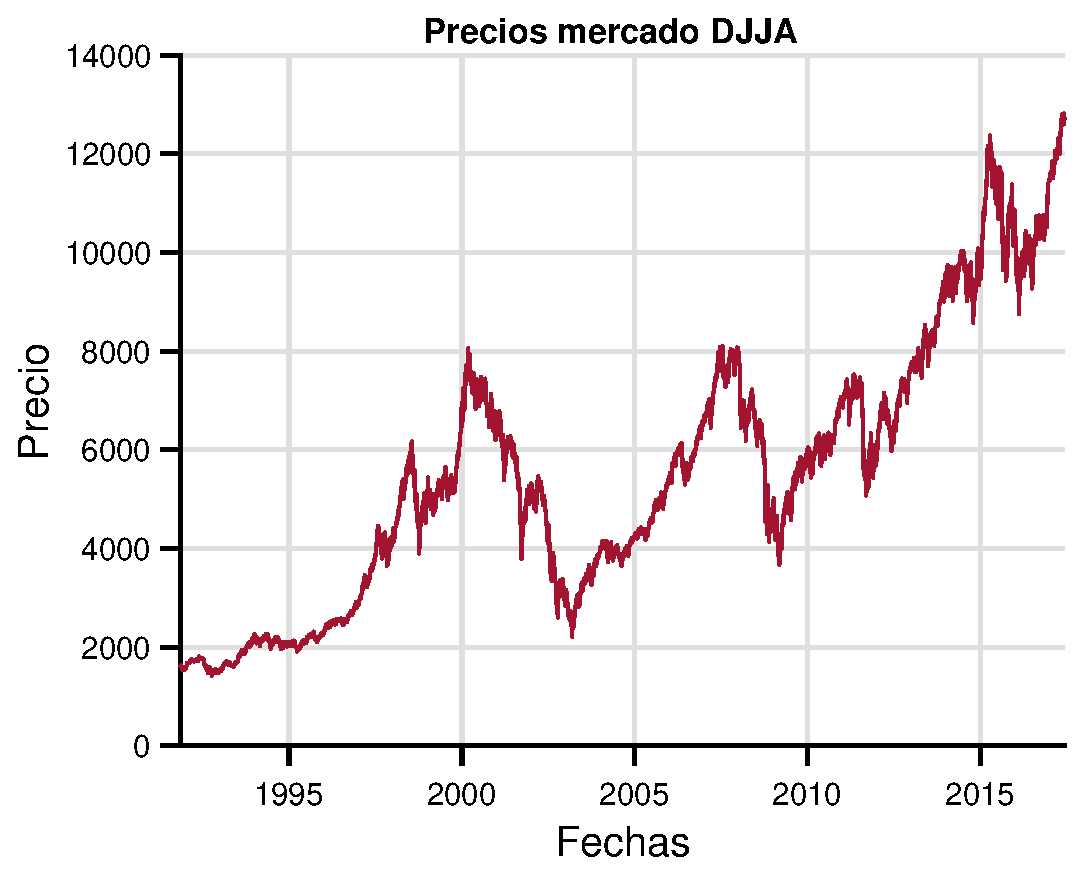
\includegraphics[width=0.7\linewidth]{figures/precioseps}
	\caption{. Evolución temporal de los precios en el mercado DJJA.}
	\label{precioseps}
\end{figure}

A partir de los datos depurados y ordenados se calcularon lo retornos como se explica en la sección \ref{Metodologia}. Se aplico el algoritmo de la Figura \ref{diagramaentropia1}. 
En la figura \ref{onlyreturnseps} se aprecia que los retornos fluctúan entorno a una media de valor cero. 
Sin embargo se aprecia que existen mínimos en el valor del retorno, como es el caso del segundo mínimo, que además es el mínimo global de todos los retornos.

\begin{figure}[h]
	\centering
	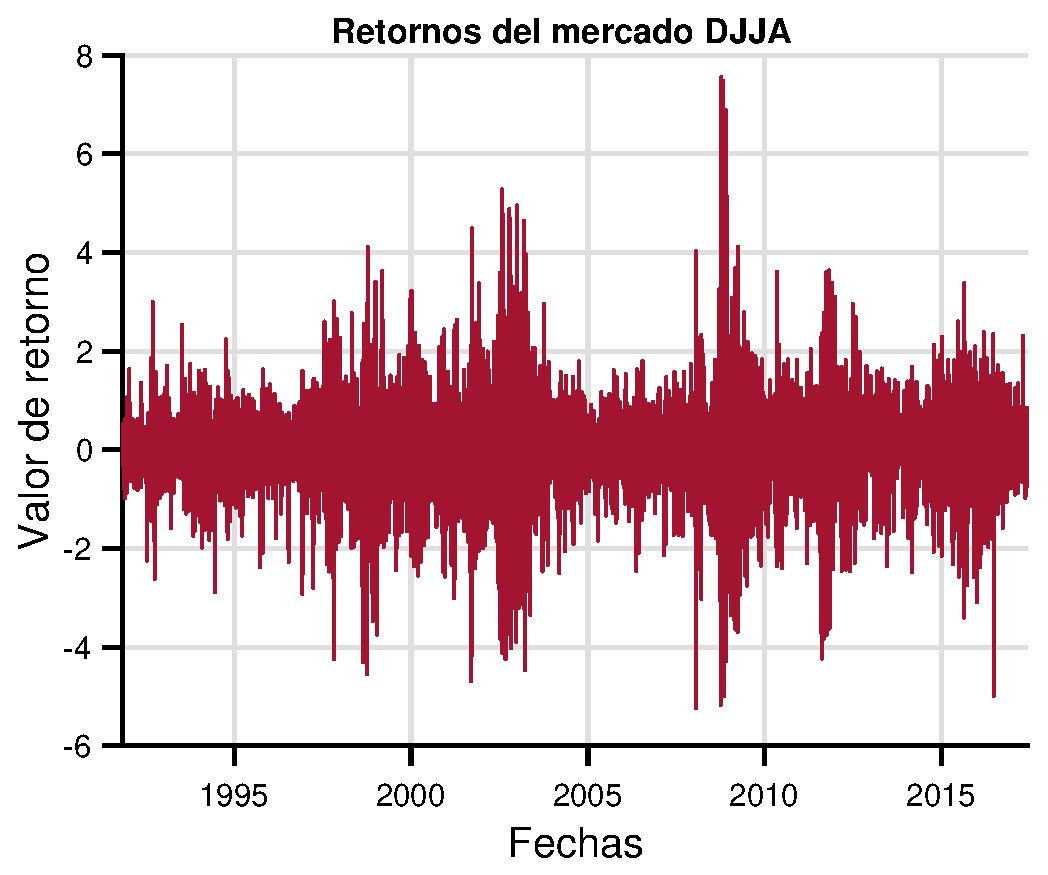
\includegraphics[width=0.7\linewidth]{figures/onlyreturnseps}
	\caption{Retornos para el mercado DJJA.}
	\label{onlyreturnseps}
\end{figure}

Posteriormente se procedio a calcular la entropia de los mercados financieros aplicando el algoritmo descrito en la Seccion \ref{sec_entropia}.
En la figura \ref{onlyentropyeps} se presentan los resultados del calculo de entropia.
Se observa que la entropía posee valores mínimos en la misma fecha (dd/mm/yyyy) del segundo mínimo que muestra el gráfico de los precios (Ver Figura \ref{precioseps}). 
Un mínimo es observado cuando varias fechas consecutivas el precio es más bajo, resultando el valor de retorno negativo. 


\begin{figure}[h]
	\centering
	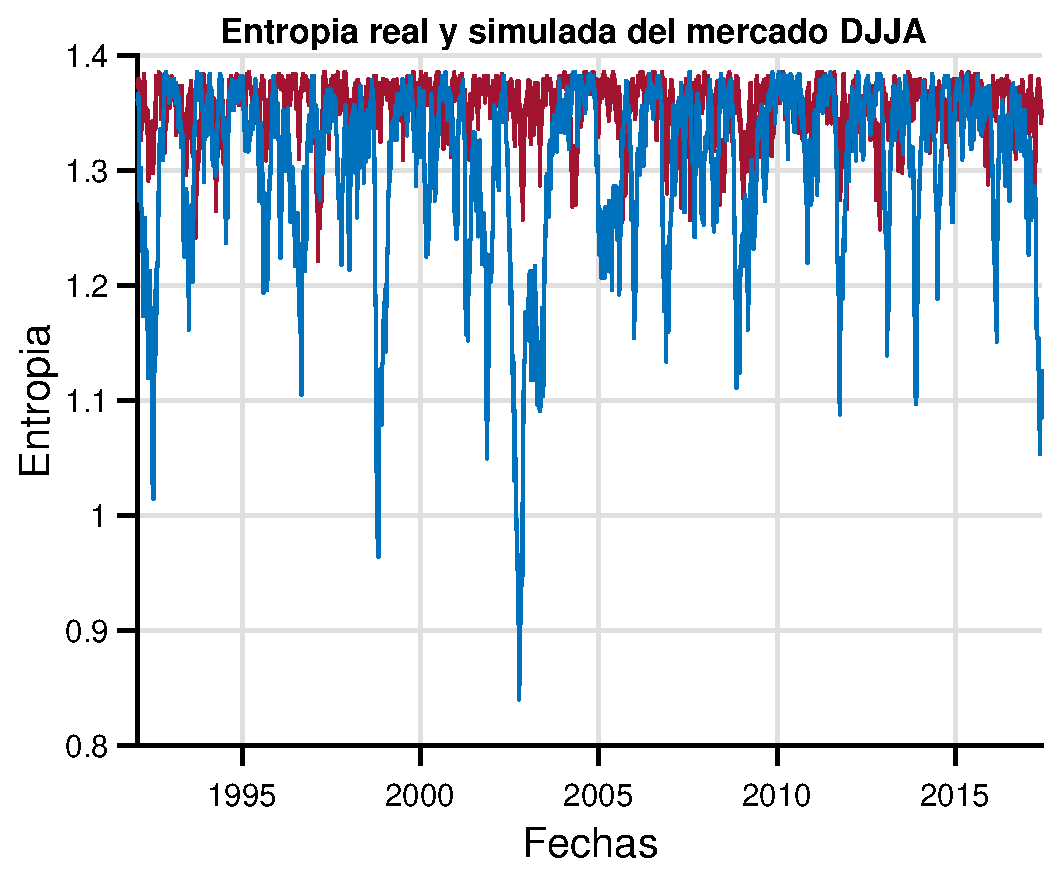
\includegraphics[width=0.7\linewidth]{figures/onlyentropyeps}
	\caption{Entropía para un mercado simulado y un mercado eficiente. Mercado real DJJA (linea azul) y mercado eficiente DJJA (linea roja).}
	\label{onlyentropyeps}
\end{figure}



\section{Resultado del cálculo de entropías con medias moviles}



\begin{figure}[h]
	\centering
	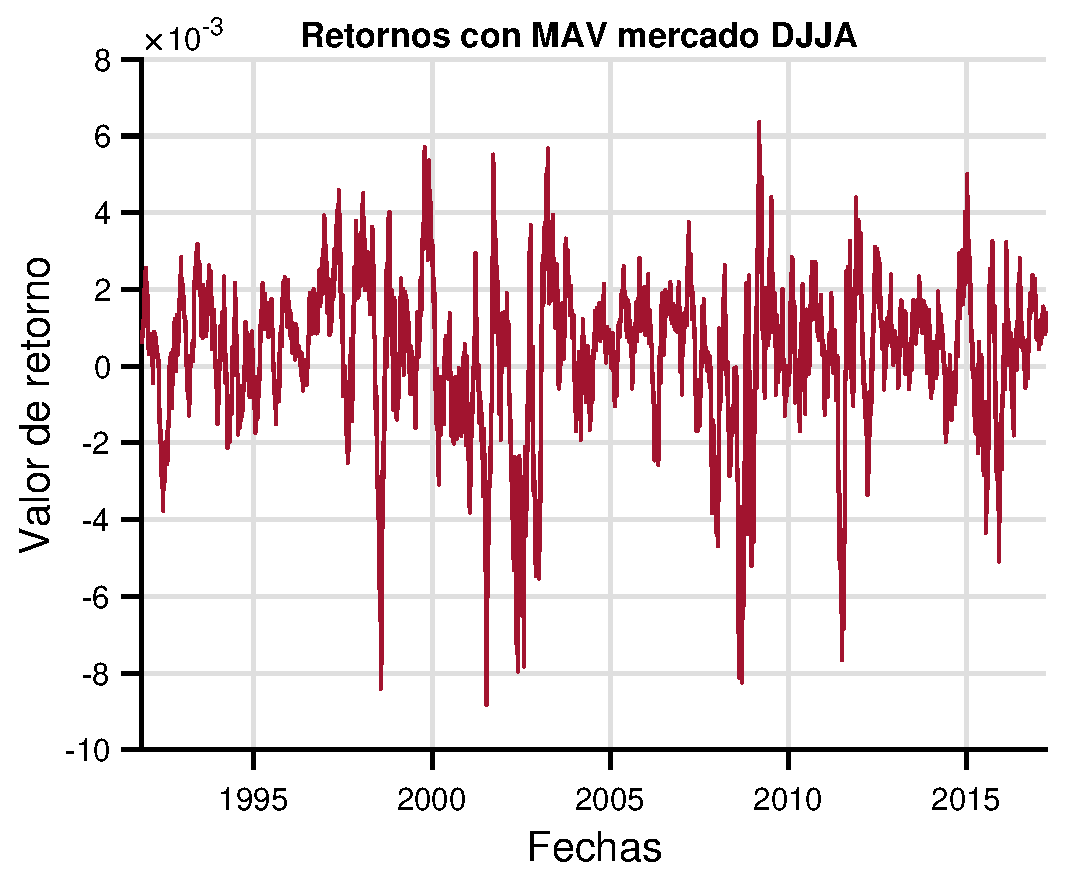
\includegraphics[width=0.7\linewidth]{figures/MAVreturnseps}
	\caption{Retornos con una media móvil de 50 días aplicada para el mercado DJJA.}
	\label{fig:mavreturnseps}
\end{figure}

En la gráfica \ref{fig:mavreturnseps} se puede apreciar que la representación de los datos es menos conglomerada debido a que se aplicó una ventana de 50 días. Este filtrado de datos permite que la gráfica conserve su comportamiento pero que sea fácil identificar puntos de interés.

\begin{figure}[h]
	\centering
	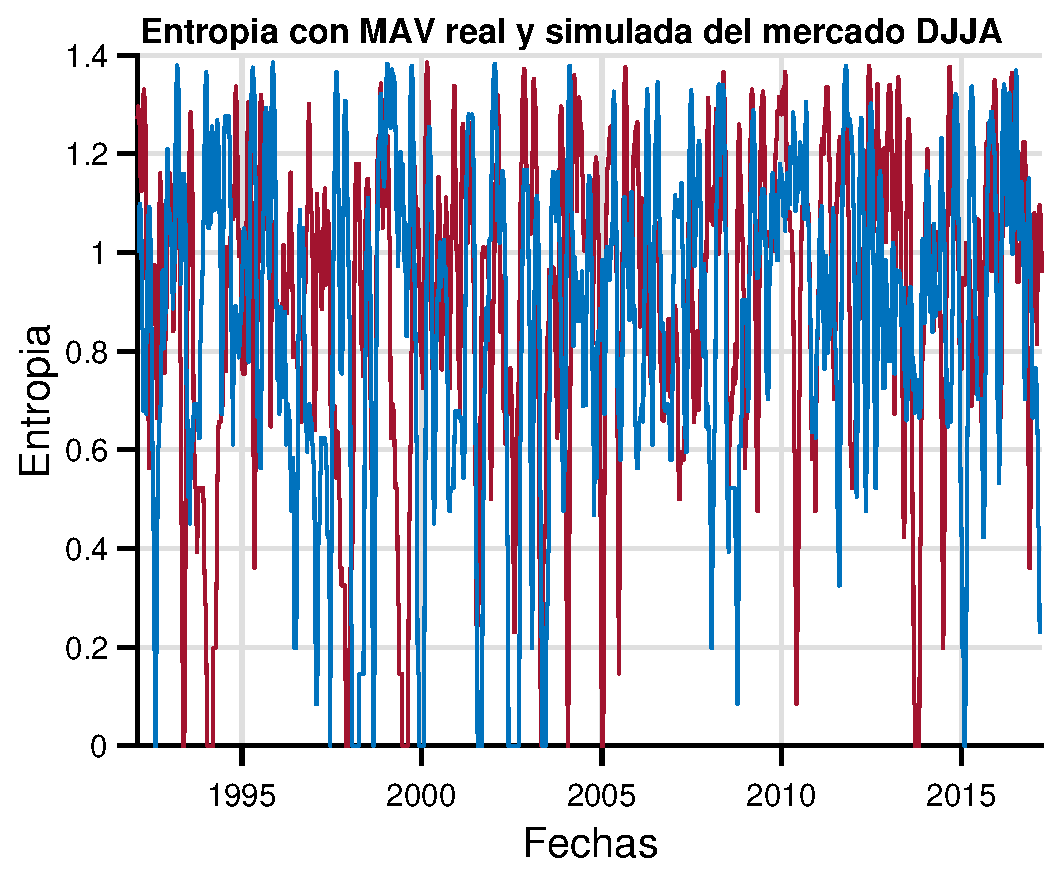
\includegraphics[width=0.7\linewidth]{figures/MAVentropy}
	\caption{Entropia del mercado real DJJA (linea azul) y un la simulacion de un mercado ideal DJJA (linea roja) con aplicación de medias móviles.}
	\label{fig:maventropy}
\end{figure}

En la gráfica de comparación (Ver figura \ref{fig:maventropy} ) entre la entropía del mercado real y la entropía del mercado simulado se tiene que cuando se simulan los retornos y se les aplica un filtro de media móvil, el cálculo de la entropía muestra que hay mínimos de la entropía con valor cero. Los retornos de datos reales muestran un comportamiento similar ya que hay más de un punto en que la entropía mínima también es cero.

\section{Simulacion de Mercado eficiente}
Se observan valores mínimos de entropía gracias a la manera en que se presentan los resultados, 
con ello comparar el comportamiento de la entropía del mercado eficiente y del mercado real con fechas, 
con o sin media móvil requiere únicamente del cálculo de un umbral que diferencie los valores de entropía que se comportan de manera gaussiana  de los que no.

Mediante la definición de un umbral que permite seleccionar con un intervalo de confianza de 95 porciento los valores de entropía mínima en los mercados. 


\section{Pruebas estadisticas}

Finalmente, se aplica una prueba estadística de distribuciones a los valores con mínima entropía, tanto de aquellos que fueron tratados con un filtro de media movil como aquellos que no. 

Recordemos que de la ecuación de la entropía de Shannon, se realiza la suma de la probabilidad del estado, multiplicado por la probabilidad del estado. Gracias a que se trabajan con probabilidades es posible graficar un histograma de las entropías, y además se puede estudiar la entropía mediante cuantiles de manera análoga con los retornos de los precios.

Calcular el intervalo de confianza para la distribución de estas entropías sale de este trabajo de tesis, ya que no se asemeja ni a una distribución normal ni a una distribución de Student, ello implicaría tener que realizar interpolaciones entre los cuantiles obtenidos tal como se muestra en el articulo A Method for Confidence Intervals of High Quantiles de Mei Ling Huang, y Xiang Raney-Yan publicado en 2021. 
%file:///D:/dark_/descarga_chrome/entropy-23-00070-v3.pdf

Por lo anterior, se propone utilizar como umbral para hallar los valores mínimos de entropía el valor del percentil 95 en vez de un íntervalo de confianza. Entre el año 2000 y 2005, se aprecia un valor mínimo en el precio, mismo que tiene impacto al estudiar la entropía.


Entonces, al realizar un gráfico que muestra la distribución de la entropía, y dado que la entropía es obtenida a partir de probabilidades, es fácil obtener cualquier cuantil (percentil 95 en el caso del intervalo de confianza), además que dicho percentil permite diferenciar aquellos valores de la entropía que son ruido de aquellos que no. 

